% Appendix B (two-cause rewrite, 2026-11): earlier attempts. Outcomes are stated in words; numbers only
% from generated files. The runs here follow the earlier protocol unless stated.
\chapter{Earlier Attempts}
\label{app:earlier}

Before the analysis of the two causes, we tried several other remedies. They did not become
part of the proposed method; however, they shaped it, and we summarize them here for
completeness. It is noted that most runs of this appendix follow an earlier protocol,
which stopped early on the test split; hence, their numbers are not comparable with those
of Chapter~\ref{ch:results}, and we state the outcomes in words unless a generated table
exists.

\section{Protecting the Layers That Drift}
\label{app:earlier-protect}

The drift analysis shows that the head and the late layers change the most
(Section~\ref{sec:c6-s1}). Our first idea was therefore to protect these parameters. We
tried a Fisher-weighted penalty that is concentrated on the head and the late layers, and
we tried freezing them after the first session. The penalty helped only together with a
replay buffer. Freezing did not help at all: with the head and the late layers frozen, the
early and middle layers, which hardly change under naive fine-tuning, drifted instead, and
the forgetting stayed at the level of naive fine-tuning. Freezing the whole model forgot
nothing and learned nothing. Hence, protecting where the drift is measured only moves the
drift to the parameters that remain trainable. This is the reason why the proposed method
does not protect parameters but shows old documents to the model again.

\section{Slot Memories Selected by the Vocabulary (DocCL and LexSlot)}
\label{app:earlier-lexslot}

Our second idea was to give every session its own small set of parameters at the head and
the late layers, and to select them by the words of the document. DocCL combined a
component-wise penalty with distillation and a small raw buffer. LexSlot replaced the
penalty with additive low-rank slots that are written once per session and selected at
test time by the overlap between the vocabulary of the document and the vocabulary of
each session. On the domain-incremental stream, where the sessions are different datasets
with different vocabularies, LexSlot came close to raw replay; however, it did so only
together with a raw replay buffer. On the class-incremental stream, where all sessions
come from one dataset and share one vocabulary, the selection has nothing to separate, and
the method stayed at the level of naive fine-tuning. We also combined the slots with
CoLaR-SBR (Table~\ref{tab:slot}); the difference to CoLaR-SBR alone changes its sign
between the runs. Hence, we dropped the slots.

\begin{table}[!htbp]
  \centering
  \caption[CoLaR-SBR with and without lexical slots]{\textbf{CoLaR-SBR with and without
  lexical slots} (AA per run: without / with, and the difference; earlier
  protocol$^{\dagger}$; ``--'': not run).}
  \label{tab:slot}
  \small% AUTO-GENERATED by scripts/rca/make_clean_tables.py -- do not edit.
\begin{tabular}{llccc}
\toprule
Scenario & Protocol & 42 & 7 & 123 \\
\midrule
CIL-CORD & gate$^{\dagger}$ & 87.6 / 90.2 ($+2.5$) & 86.3 / 89.7 ($+3.5$) & 90.1 / 89.2 ($-0.9$) \\
Mixed & gate$^{\dagger}$ & 89.7 / 88.5 ($-1.2$) & -- / 90.0 & -- / 90.3 \\
DIL & gate$^{\dagger}$ & 86.8 / 87.2 ($+0.5$) & 84.8 / 87.2 ($+2.5$) & 87.1 / 86.6 ($-0.5$) \\
\bottomrule
\end{tabular}

\end{table}

\section{Routing with Prompts}
\label{app:earlier-routing}

Prompt-based methods keep the encoder frozen and select prompts for a test sample. We
examined whether a better selection would make them work on documents: a sparse selection
by the words of the document identifies the session far more reliably than the dense
query of the published methods. However, the accuracy did not follow. Even with the right
prompts, the shared head is retrained by every session and drifts; hence, the selection
was not the bottleneck. This agrees with the results of CODA-Prompt in
Table~\ref{tab:main}.

\section{Memories That Summarize}
\label{app:earlier-summary}

Before CoLaR, we tried to replace the stored documents with summaries of their features:
a low-rank subspace of all features, one Gaussian per class, and centroids of real
features. On the domain-incremental stream, all of them fell to the level of naive
fine-tuning, whereas replaying the real activations of whole documents came close to raw
replay (Figure~\ref{fig:falsification-ladder}). A control explains why: when the same real
features are replayed without the positions and the neighbours of their document, they
also fail. We also replayed public documents with pseudo-labels instead of stored ones;
this recovered a session only when the public documents resembled its documents. Besides,
the features of all documents together are close to full rank, so a small subspace cannot
keep them, whereas the features of one document are low-rank. These findings led to the
design of CoLaR: keep whole documents, and compress each document on its own
(Section~\ref{sec:m-colar}).

\begin{figure}[!htbp]
  \centering
  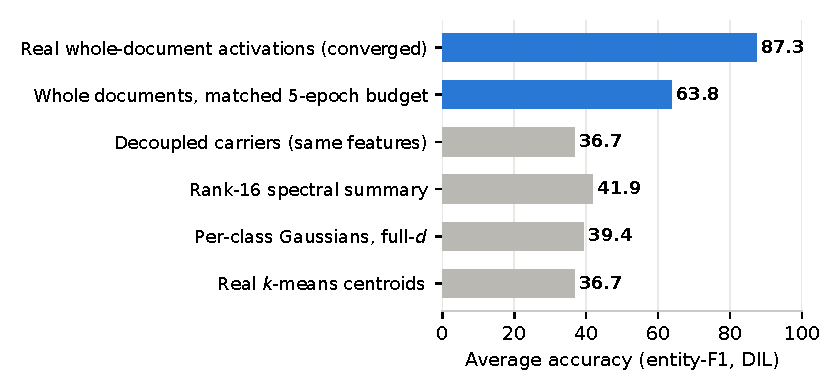
\includegraphics[width=0.8\textwidth]{paper/falsification_ladder.pdf}
  \caption[Memories that summarize against whole documents]{\textbf{Memories that
  summarize against whole documents} (DIL, one run each, earlier protocol). Only the
  replay of whole documents keeps the accuracy.}
  \label{fig:falsification-ladder}
\end{figure}
